\chapter{Research Plan}

In my project plan I stated that "I will demonstrate my master level by understanding and simulating the dynamics of a 6 axis Robot arm."\cite{ProjectPlan}

This should be done by creating a model of the robot arm. 
To create the model of the robot arm, a view on existing literature is necessary to lay out the best approach. 

To start the literature review, a set of first keywords was needed. Through an expert interview with my company supervisor, who had already supervised other thesis projects in the domain of robotics, a list of keywords to start with was obtained. Not all of these keywords were immediately clear, so it was necessary to find clear definitions for these. With the help of scientific databases and search engines, papers for these definitions could be found.


	%\caption{Keywords to begin with}
	\begin{itemize} [leftmargin=3cm]
	\item [6 axis robot] serial 6 degree of freedom robots (\cite{6axisRobot} with HANQuest)
		\item [industrial robot arm]  some form of jointed structure  achieved by the linking of a number of rotary and/or linear motions or joints( \cite{IndustrialRobotArm} with ScienceDirect)
		\item [inverse kinematics]  mathematical process of recovering the movements of an object with kinematic equaions to determine the joint paramters that provide a desired position for each of the robot's end effectors (\cite{InvKinDef} with Wikipedia)
		\item[{\parbox[t]{0.2\linewidth}{Peter Corke \\ robotics toolbox}}]Matlab toolbox for the study and simulation of classical arm-type robotics, for example such things as kinematics, dynamics, and  trajectory generation (\cite{CorkeRoboticsToolbox} with Google search)
		\item [Motion planning]  find a sequence of valid configurations that moves the robot from the source to destination (\cite{MotionPlanning} with Google search)
		\item [robot dynamics] relationship between the forces acting on a robot mechanism and the accelerations they produce (\cite{RobotDynamics}, with Scholarpedia)
		\item [ROS]  framework for writing robot software. It is a collection of tools, libraries, and conventions that aim to simplify the task of creating complex and robust robot behaviour across a wide variety of robotic platforms. (\cite{ROS} with Google search )
		%manual linebreak in item label
%		\item[{\parbox[t]{0.2\linewidth}{force here \\ a linebreak}}] Some text right of the label 
\end{itemize} 



Starting from the source for the industrial robot arm, it was determined, that the FANUC 210F is an articulated robot.


















%In the module Systems modelling of the master course control systems at HAN, the 4+1 approach \ref{4+1} was presented. 
%
%\begin{figure}[H]
%	\centering
%	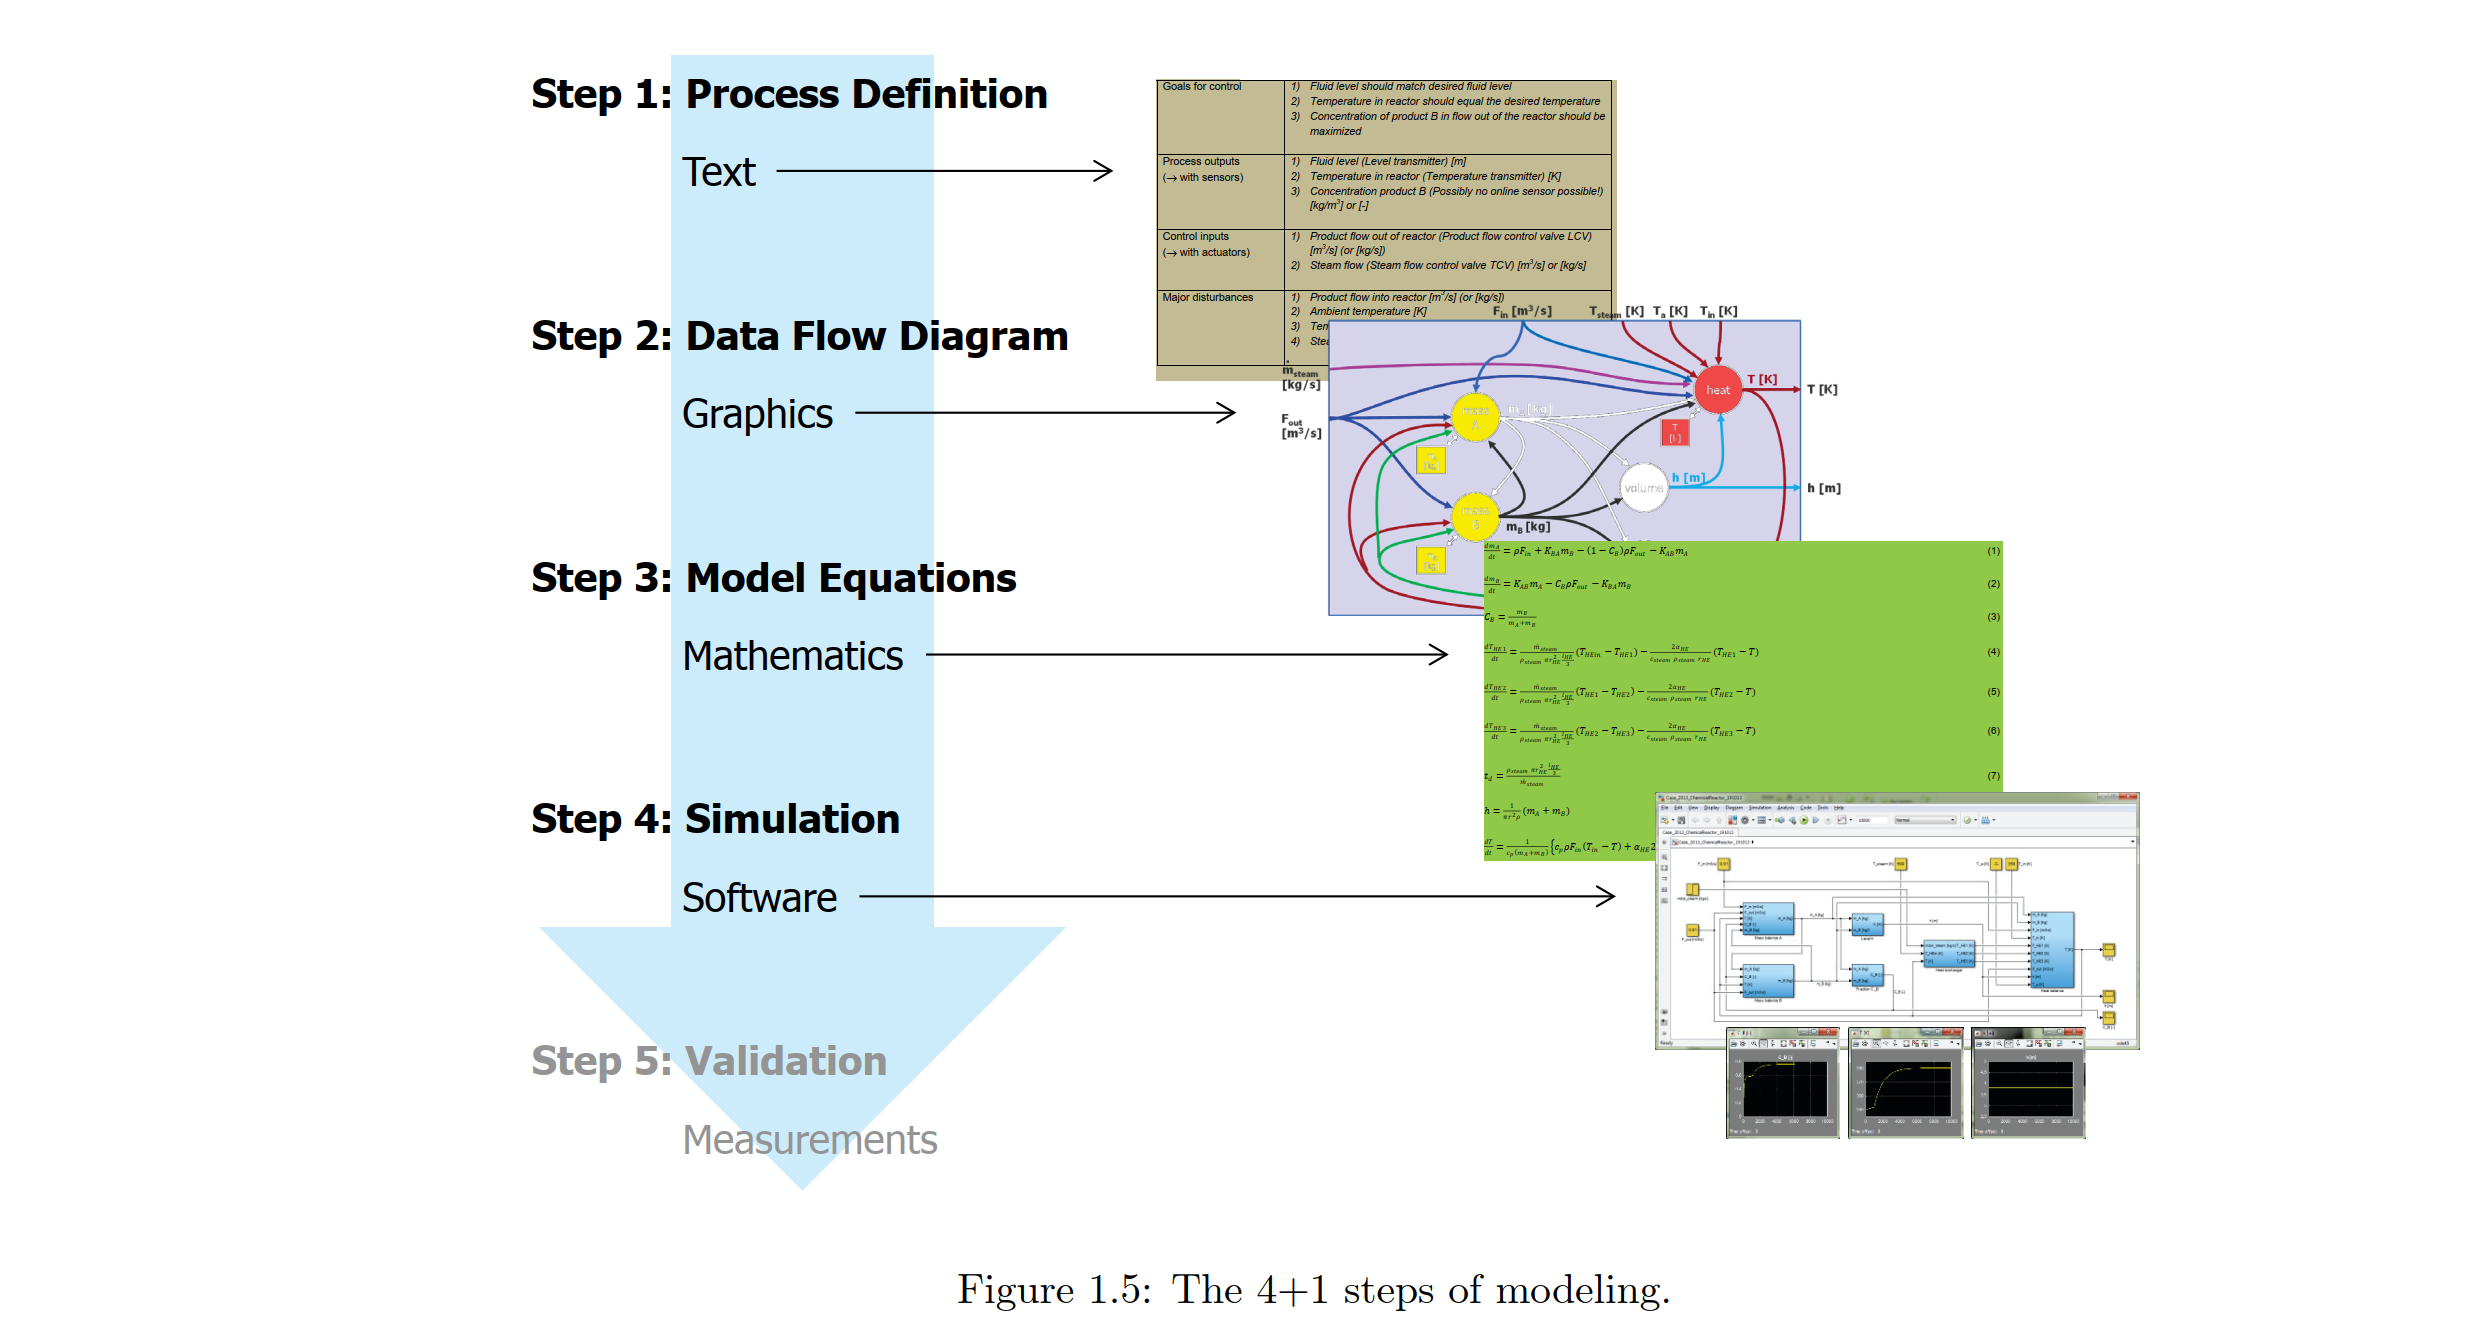
\includegraphics[
%	width=1\linewidth,
%	height=\paperheight,
%	keepaspectratio,
%	]{4+1Approach}
%	\caption{4+1 steps of modeling}
%	\label{fig:4+1}
%\end{figure}
%\pagestyle{empty}
%
%Starting from the process definition, model equations are derived with the help of a data flow diagram that lead to a simulation in software, e.g. Matlab. If possible, in the "+1" step, this model is validated with the real system.
%
%\section{Process Defintion}
%For object manipulation and other tasks, a robot arm needs to move to desired positions or track a given path. As the process focusses on the endpoint position of the robot arm, the process output can be defined as the xyz-position of the toolhead in space. The input, which can be used to control this output is the desired position. Another input that effects the output are objects attached to or carried by the robot arm. These can be considered disturbance inputs. From this, the process definition can be derived as seen in \ref{tab:ProcessDefinition}.
%
%\begin{table}[H]
%	\centering
%	\caption{Process Definiton}
%	\begin{tabular}{ll}
%		Goal for control:& Endpoint position of Robot arm   \\
%		Process output: & Endposition of Robot arm
%		 (sensor: measured with pulse encoders on the axes)   \\
%		Control inputs: & Electric power to the actuators
%		 (actuator: motor)  \\
%		Major disturbance & Carried object  
%	\end{tabular}
%\label{tab:ProcessDefinition}
%\end{table}